\section{Methodology}\label{sec:pcsregression:methodology}
In this work, we propose a strategy for automatically identifying low-dimensional strain models for continuum robots directly from shape trajectories, as outlined in Figure \ref{fig:pcsregression:overall_diag}.
We assume that we have access to the poses of $N$ markers along the backbone that represent a discretized shape description of the soft robot.
% These could be provided by, for example, a motion capture system or, as done in this work, extracted using computer vision techniques from images.
In this work, we primarily focus on the planar case, where we extract SE(2) poses using computer vision techniques. However, the proposed \emph{Kinematic Fusion} approach, along with the \emph{Dynamic Regression and Strain Sparsification} strategy, can be extended to 3D scenarios with SE(3) inputs. While obtaining consistent and unoccluded SE(3) poses solely from vision-based information in 3D can be challenging, it is feasible~\citep{zheng2024vision}. Additionally, SE(3) pose measurements can always be acquired through other proprioceptive~\citep{rosi2022sensing} or exteroceptive methods, such as motion capture systems.

The goal is now to identify kinematic and dynamical models that allow (a) to represent the shape with 
$n_\mathrm{s}$ \gls{PCS} segments~\citep{renda2018discrete}, where necessarily the final $n_\mathrm{s} \ll N$, and (b) to predict the future shape evolution of the soft robot.
We tackle this task by (i) identifying a low-dimensional parametrization (e.g., number of constant strain segments, the length of each segment, etc.) of the kinematics over a series of static snapshots and (ii) identifying the parameters of the Lagrangian model and simultaneously eliminating strains from the model that do not have a significant effect on the shape evolution.
We refer to component (i) as the \emph{Kinematic Fusion} algorithm, as it is an iterative approach to merge parts of the backbone that exhibit a similar strain into constant strain segments.
The component (ii), named \emph{Dynamic Regression \& Strain Sparsification} algorithm, is an iterative procedure that, at each iteration, first regresses in closed-form the coefficients of the dynamic using linear least-squares and then eliminates strains from the dynamic model if the stiffness associated with a strain exceeds a given threshold. The intuition here is that strain would oscillate at very high frequencies, which are usually not relevant for practical control, and that it would take very high forces to introduce a significant deflection in the strain.
The output of our approach is low-dimensional kinematic and dynamical models that preserve the physical \& \gls{PCS} strain model structures.

% We start with images of multiple trajectories, which are processed using computer vision (CV) to estimate the poses of $N$ markers along the soft robot. An initial $N$-segment \gls{PCS} model is considered to obtain the robot's configuration through inverse kinematics. We employ a kinematic fusion procedure to reduce it to $m$ segments while preserving accuracy. Finally, dynamic model identification is performed, estimating the dynamic parameters and eliminating negligible strains, resulting in a low-dimensional model suitable for control applications.

\begin{figure}
    \centering
    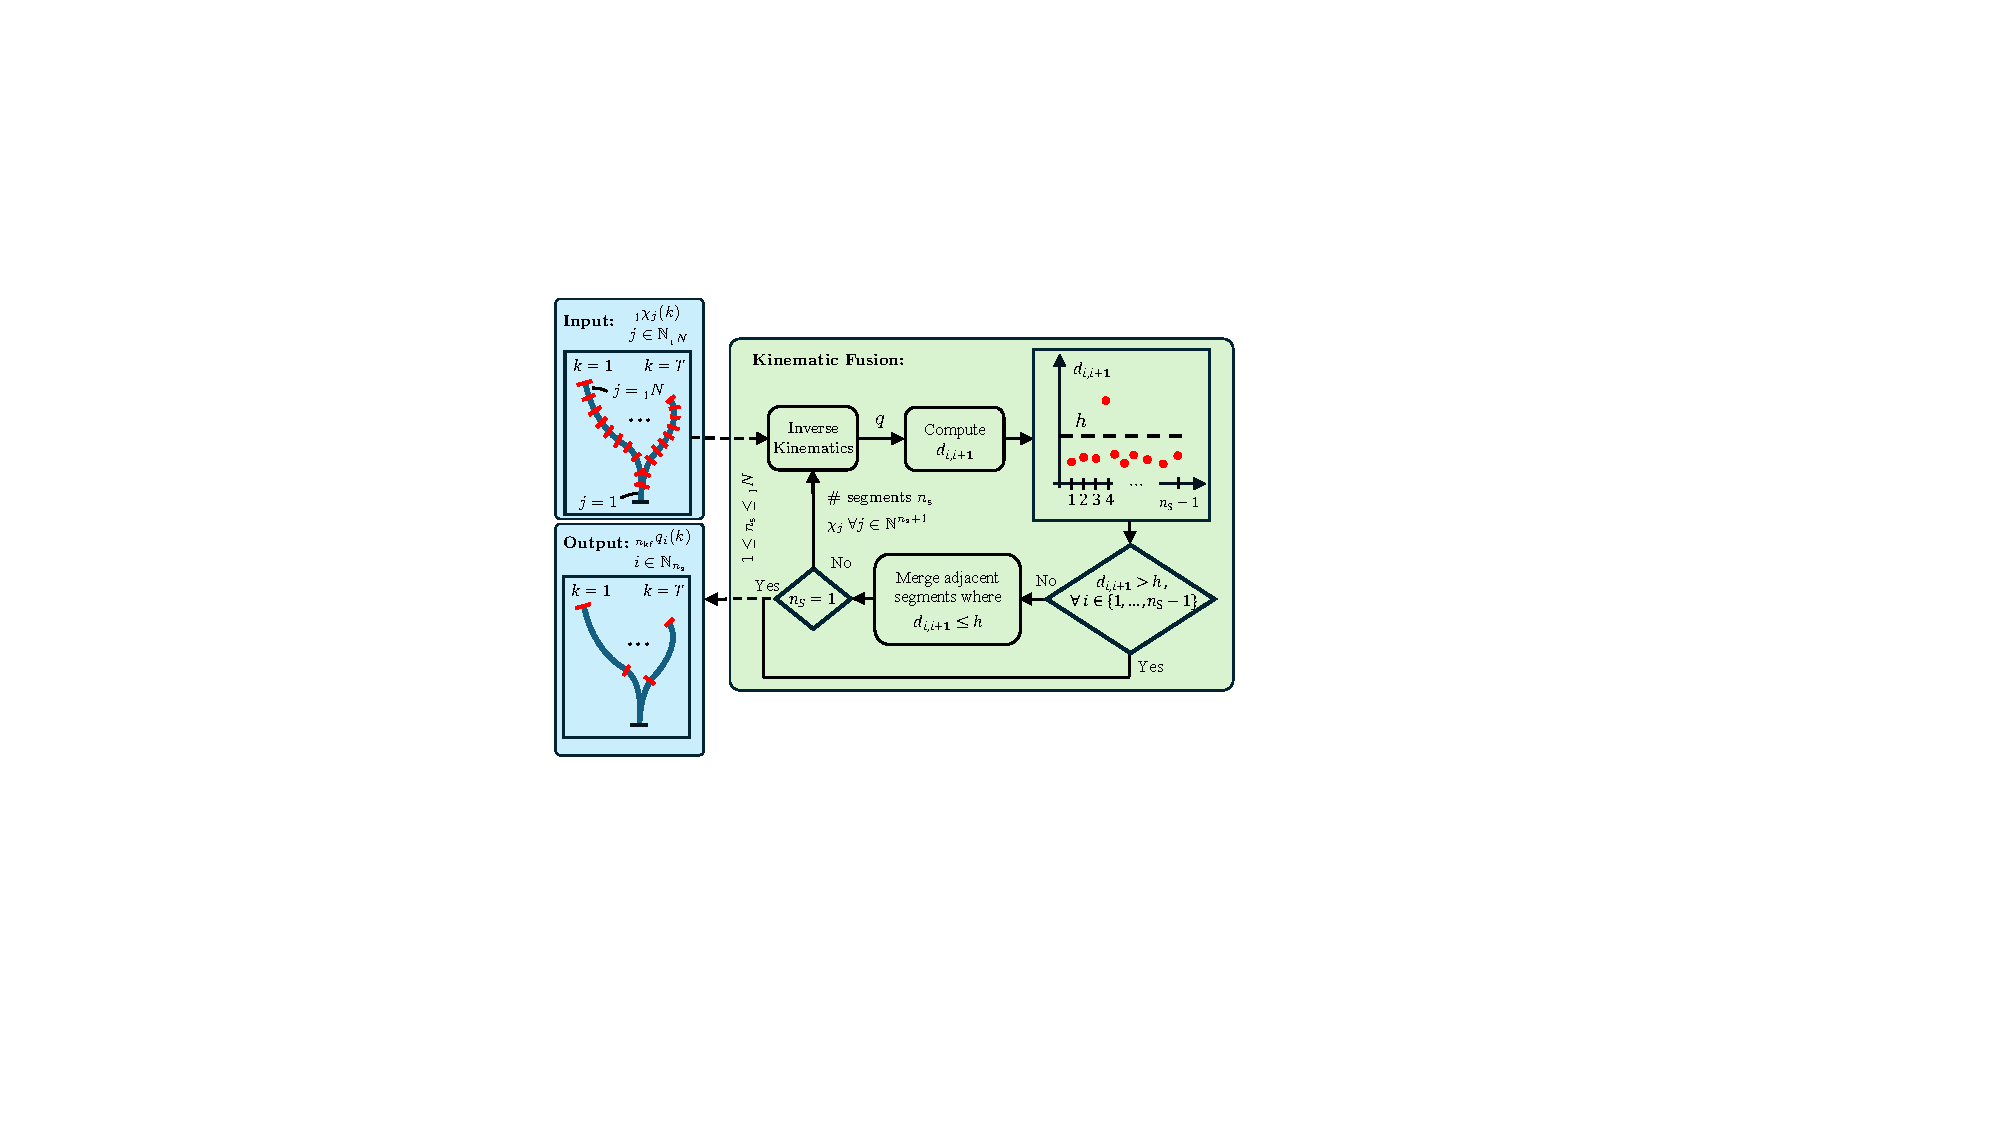
\includegraphics[width=0.7\linewidth]{pcsregression/figures/diagram_kinematic_fusion_v3_cropped.pdf}
    \caption{Schematic of the kinematic fusion algorithm. As inputs serve a sequence of $N$ discrete poses along the backbone of the soft robot. Next, we execute inverse kinematics in closed form with a $n_\mathrm{s} = N-1$ segment \gls{PCS} model to identify the (unmerged) configuration of the robot. Initially, each constant strain segment connects two neighboring backbone poses. Subsequently, we compute a strain similarity measure $\bar{d}_{i,i+1}$ between each pair of adjacent segments. If segments exhibit a similar strain (i.e., the metric falls below a threshold $h$), we merge them into one constant strain segment. This process is repeated until no more merging is possible, resulting in a kinematic model with (hopefully) fewer segments: $1 \leq n_\mathrm{s} \leq N-1$.}
    \label{fig:pcsregression:kin_regr}
\end{figure}

\subsection{Kinematic Fusion}
As previously introduced, the algorithm is provided for each training dataset sample $k \in \{1, \dots, T\}$ with $N$ pose measurements $\chi$ and associated backbone abscissas $s \in \mathbb{R}^N$ distributed along the backbone of the soft robot.
Therefore, we initialize at $l=1$: $\presub{1}{N} = N$ and $\presub{1}{\chi} = \chi$, where $l \in \mathbb{N}_{\geq 1}$ denotes the iteration index.

At the beginning of each iteration, we leverage the closed-form inverse kinematics to compute the configuration $\presub{l}{q} = \rho(\presub{l}{\chi}, \presub{l}{s}) $ of a $\presub{l}{n}_\mathrm{s} = \presub{l}{N} - 1$ segment \gls{PCS} model. We now compute between each of the total $\presub{l}{n}_\mathrm{s} - 1$ segment pairs, the following normalized strain similarity measure
\begin{equation}
    \presub{l}{\bar{d}}_{i,i+1} = \frac{1}{T} \sum_{k=1}^T \left \lVert \frac{\presub{l}{q}_{i+1}(k) - \presub{l}{q}_i(k)}{q^\mathrm{max} - q^\mathrm{min}} \right \rVert_2, \quad \forall i \in \{1, \presub{l}{n}_\mathrm{s}-1 \},
\end{equation}
where
\begin{equation}
    q^\mathrm{min} = \min_{i \in \mathbb{N}_{n}, k \in \mathbb{N}_T} q_i(k), 
    \qquad 
    q^\mathrm{max} = \max_{i \in \mathbb{N}_{n}, k \in \mathbb{N}_T} q_i(k),
\end{equation}
are the minimum and maximum configuration values across the dataset, respectively. This normalization is necessary as strains usually exhibit vastly different magnitudes. For example, the bending strains are usually more than one order of magnitude larger than the axial strains.
We keep all segment pairs with $\presub{l}{\bar{d}}_{i,i+1} > h$, where $h$ is a tunable threshold, separate. Oppositely, we merge all neighboring/adjacent segments with $\presub{l}{\bar{d}}_{i,i+1} \leq h$ into one single segment of constant strain.
If indeed $\exists \: i \in \{ \mathbb{N}_{\presub{l}{n}_\mathrm{s}} | \presub{l}{\bar{d}}_{i,i+1} < h \}$, then then kinematic model is reduced to $\presub{l+1}{n}_\mathrm{s}$ segments, where $\presub{l+1}{n}_\mathrm{s} < \presub{l}{n}_\mathrm{s}$.
As a final step of the iteration, we now subsample the Cartesian poses $\presub{l+1}{\chi}$ and the associate backbone coordinates $\presub{l+1}{s}$ such that they only contain the tip of each of the fused segments.
% As a final step of the iteration, we update the Cartesian poses using the forward kinematics to correspond to the tip of each segment: $\presub{l+1}{\chi} = \pi(\presub{l+1}{q})$

The kinematic fusion step is repeated with $l = l + 1$ for $n_\mathrm{kf}-1$ iterations until no more merging is possible, which can occur either if $\presub{n_\mathrm{kf}}{{\bar{d}}}_{i,i+1} > h \: \forall i \in \{1, \presub{n_\mathrm{kf}}{n}_\mathrm{s}-1 \}$ (i.e., the strain similarity measure is larger than $h$ for every pair of segments) or the model gets reduced to a single segment (i.e., $\presub{n_\mathrm{kf}}{n}_\mathrm{s} = 1$).
We illustrate the kinematic fusion algorithm in Fig.~\ref{fig:pcsregression:kin_regr}, and an example of the thresholding is visualized in Fig.~\ref{fig:pcsregression:results:kinematic_fusion:pcs_ns-2}.


% To develop a \gls{PCS} kinematic model for a generic soft robot, it is necessary to determine the number of segments and the length of each segment. In this work, we achieve this by means of a strain-based algorithm.

% Given that we now have access to the poses of $N$ equally distant cross-sections along the robot, we initialize an $N$-segment \gls{PCS} kinematic model, with nodes positioned at the center of the $N$ cross-sections. Essentially, each of the $N$ tracked cross-sections will consist of a segment's end section. We apply the closed-form inverse kinematics from \eqref{eq:pcsregression:inverse_kin_pcs} to map the Cartesian poses $\chi_i$ into configuration variables $q_i$. To avoid the numerical instabilities near the straight configuration ($\theta=0$), a small $\varepsilon$ is added to the bending angle. It is important to note that $[p_x,p_y,\theta]$ in \eqref{eq:pcsregression:inverse_kin_pcs} must be written with respect to the previous frame ${S_{i-1}}$. However, the computer vision step outputs all the poses $\chi_i$ with respect to the fixed frame attached to the base of the soft robot. Therefore, a mapping must be applied to go from $\prescript{0}{}{\chi}_i$ into $\prescript{i-1}{}{\chi}_i$. This is achieved using the composition operation
% \begin{align}
%     \prescript{i-1}{}{H}_i = \prescript{i-1}{}{H}_0 \prescript{0}{}{H}_i = \left(\prescript{0}{}{H}_{i-1}\right)^{-1} \prescript{0}{}{H}_i \,,
% \end{align}
% where $\prescript{0}{}{H}_i$ is the homogeneous transformation matrix that represents pose $\prescript{0}{}{\chi}_i$. For the planar case, this is given by
% \begin{align}
%     \prescript{0}{}{H}_i = \begin{bmatrix}
%         \cos{\theta_i} & -\sin{\theta_i} & p_x^i \\ \sin{\theta_i} & \cos{\theta_i} & p_y^i \\ 0 & 0 & 1
%     \end{bmatrix}\,.
% \end{align}
% Once $\prescript{i-1}{}{H}_i$ has been computed, $\prescript{i-1}{}{\chi}_i$ can be extracted from the matrix entries.

% After computing the sequence of configurations for the $N$ initial segments, we employ a recursive algorithm to determine the final number of segments $m$, where $m<N$. The idea is that adjacent segments that have similar strain trajectories (i.e., deform similarly) can be merged together and considered a single segment. Note that each local strain has distinct units (bending strain has units $\mathrm{m^{-1}}$, while shear and axial strains are unitless). In order to compute a metric that measures strain similarity over the entire strain-space, we apply a normalization by scaling each strain relative to their maximum values. In this work, the bending strain is not greater than $60 \,\mathrm{m^{-1}}$, while shear and axial strains achieve maximum values of $30\,\mathrm{\%}$.

% The metric to measure strain similarity is the average strain-space (euclidean) distance between pairs of consecutive segments,
% \begin{align}
%     \bar{d}_{i,i+1} = \frac{1}{T} \sum_{k=1}^T \left\| \bar{q}_i (k) - \bar{q}_{i+1} (k) \right\|\,,
% \end{align} 
% where $\bar{q}_i$ represent the $i$-th segment's scaled strains. 
% %Note that this metric is dependent on the strain magnitudes, which differ across the strain-space since local strains have distinct units (bending strain has units $\mathrm{m^{-1}}$, while shear and axial strains are unitless). Therefore, to ensure a more even contribution to the similarity metric from each strain, these are first scaled relative to their maximum values. In this work, the bending strain is not greater than $60 \,\mathrm{m^{-1}}$, while shear and axial strains achieve maximum values of $30\,\mathrm{\%}$.

% We compute this average strain distance for each pair of adjacent segments. For a kinematic model with $n_S$ segments, this yields $n_S-1$ pairs. If the distance $\bar{d}_{i,i+1}$ for the $i$-th pair is below or equal to a pre-defined threshold $h$, segments $i$ and $i+1$ will be grouped into a single segment. Otherwise, the segments remain separate. This results in a new \gls{PCS} kinematic model with fewer segments. Figure \ref{fig:pcsregression:kin_regr} illustrates this procedure. The configuration of each new merged segment is determined by performing a one-segment inverse kinematics on the distal ends of the merged segment.
% % averaging the (nonscaled) strains of its $c$ constituent segments, weighted by their lengths,
% % \begin{align}
% %     q_{\text{merged}} = \frac{\sum_{j=1}^c q_j L_{0,j}}{\sum_{j=1}^c L_{0,j}} \,.
% %\end{align}


% This sequence is repeated until no more merging is possible, which can occur either if $\bar{d}_{i,i+1}$ is larger than $h$ for every pair of segments or the model gets reduced to a single segment. Algorithm \ref{alg:kin_regression} illustrates an overview of all the steps.

% \begin{algorithm}
% \caption{Kinematic Regression}
% \label{alg:kin_regression}
% \begin{algorithmic}[1]
% % \REQUIRE Poses $\prescript{0}{}{\chi}_i (k)$ \COMMENT{$i=1,...,N$}
% \REQUIRE Configurations $q_i (k)$  \COMMENT{$i=1,...,N$}
% \ENSURE Configurations $q_i (k)$ \COMMENT{$i=1,...,m\,\,(m<N)$}

% % \FOR{each frame $k=1$ \TO $T$}
% % \FOR{each cross-section $i=1$ \TO $N$}
% % \STATE $\prescript{0}{}{T}_i \gets \prescript{0}{}{\chi}_i$
% % \STATE $\prescript{i-1}{}{T}_i = ( \prescript{0}{}{T}_{i-1} )^{-1} \prescript{0}{}{T}_i$
% % \STATE $\prescript{i-1}{}{\chi}_i \gets \prescript{i-1}{}{T}_i$
% % \STATE $q_i \gets \text{IK}(\prescript{{i-1}}{}{\chi}_i) $
% % \ENDFOR
% % \ENDFOR
% % \STATE
% \REPEAT
%     \STATE $\bar{q}_i \gets q_i / q_{\text{max}}$ \COMMENT{Scale $q_i$}
%     \STATE \textit{merge\_candidates} $\gets [\,]$
%     \STATE \textit{current\_merge} $\gets [1]$
%     \FOR{$i=1$ \TO $n_S-1$}
%         \STATE $\bar{d}_{i,i+1} \gets \frac{1}{T} \sum_{k=1}^T \left\| \bar{q}_i (k) - \bar{q}_{i+1} (k) \right\|$
%         \IF{$\bar{d}_{i,i+1} \leq h$}
%             \STATE Append $i+1$ to \textit{current\_merge}
%         \ELSE 
%         \STATE Append \textit{current\_merge} to \textit{merge\_candidates}
%         \STATE Reinitialize \textit{current\_merge} $\gets [i+1]$
%         \ENDIF
%     \ENDFOR
%     % \FOR{each segment pair $(i, i+1)$}
%     %     \STATE Compute $\bar{d}_{i,i+1}$
%     %     \IF{$\bar{d}_{i,i+1} < p$}
%     %         \STATE Add $(i,i+1)$ to \textit{merge\_candidates}
%     %     \ELSE 
%     %     \STATE Keep $(i,i+1)$ as separate segments 
%     %     \ENDIF
%     % \ENDFOR
%     \STATE
%     \FOR{each group in \textit{merge\_candidates}}
%     % \STATE \COMMENT{$m$ constituent segments with lengths $L_{0,j}$}
%     %\STATE \COMMENT{Compute $q_{\text{merged}}$ by averaging the configurations of the constituent segments $1,2,...,m$, weighted by their lengths $L_{0,j}$} 
%     % \STATE $q_{\text{merged}} = \sum_{j=1}^{c} (q_{j} L_{0,j} /  L_{0,j})$
%     \STATE $q_{\text{merged}} = \text{IK}(\prescript{{\text{init}}}{}{\chi}_{\text{end}})$
%     \STATE \COMMENT{$\prescript{{\text{init}}}{}{\chi}_{\text{end}}$ is the pose of the end section of the merged segment relative to the initial section}
%     \ENDFOR
% \UNTIL{$n_S=1$ \OR $\bar{d}_{i,i+1}>h\,, \forall\, i \in [1,n_S-1]$}
% \end{algorithmic}
% \end{algorithm}

\begin{figure}
    \centering
    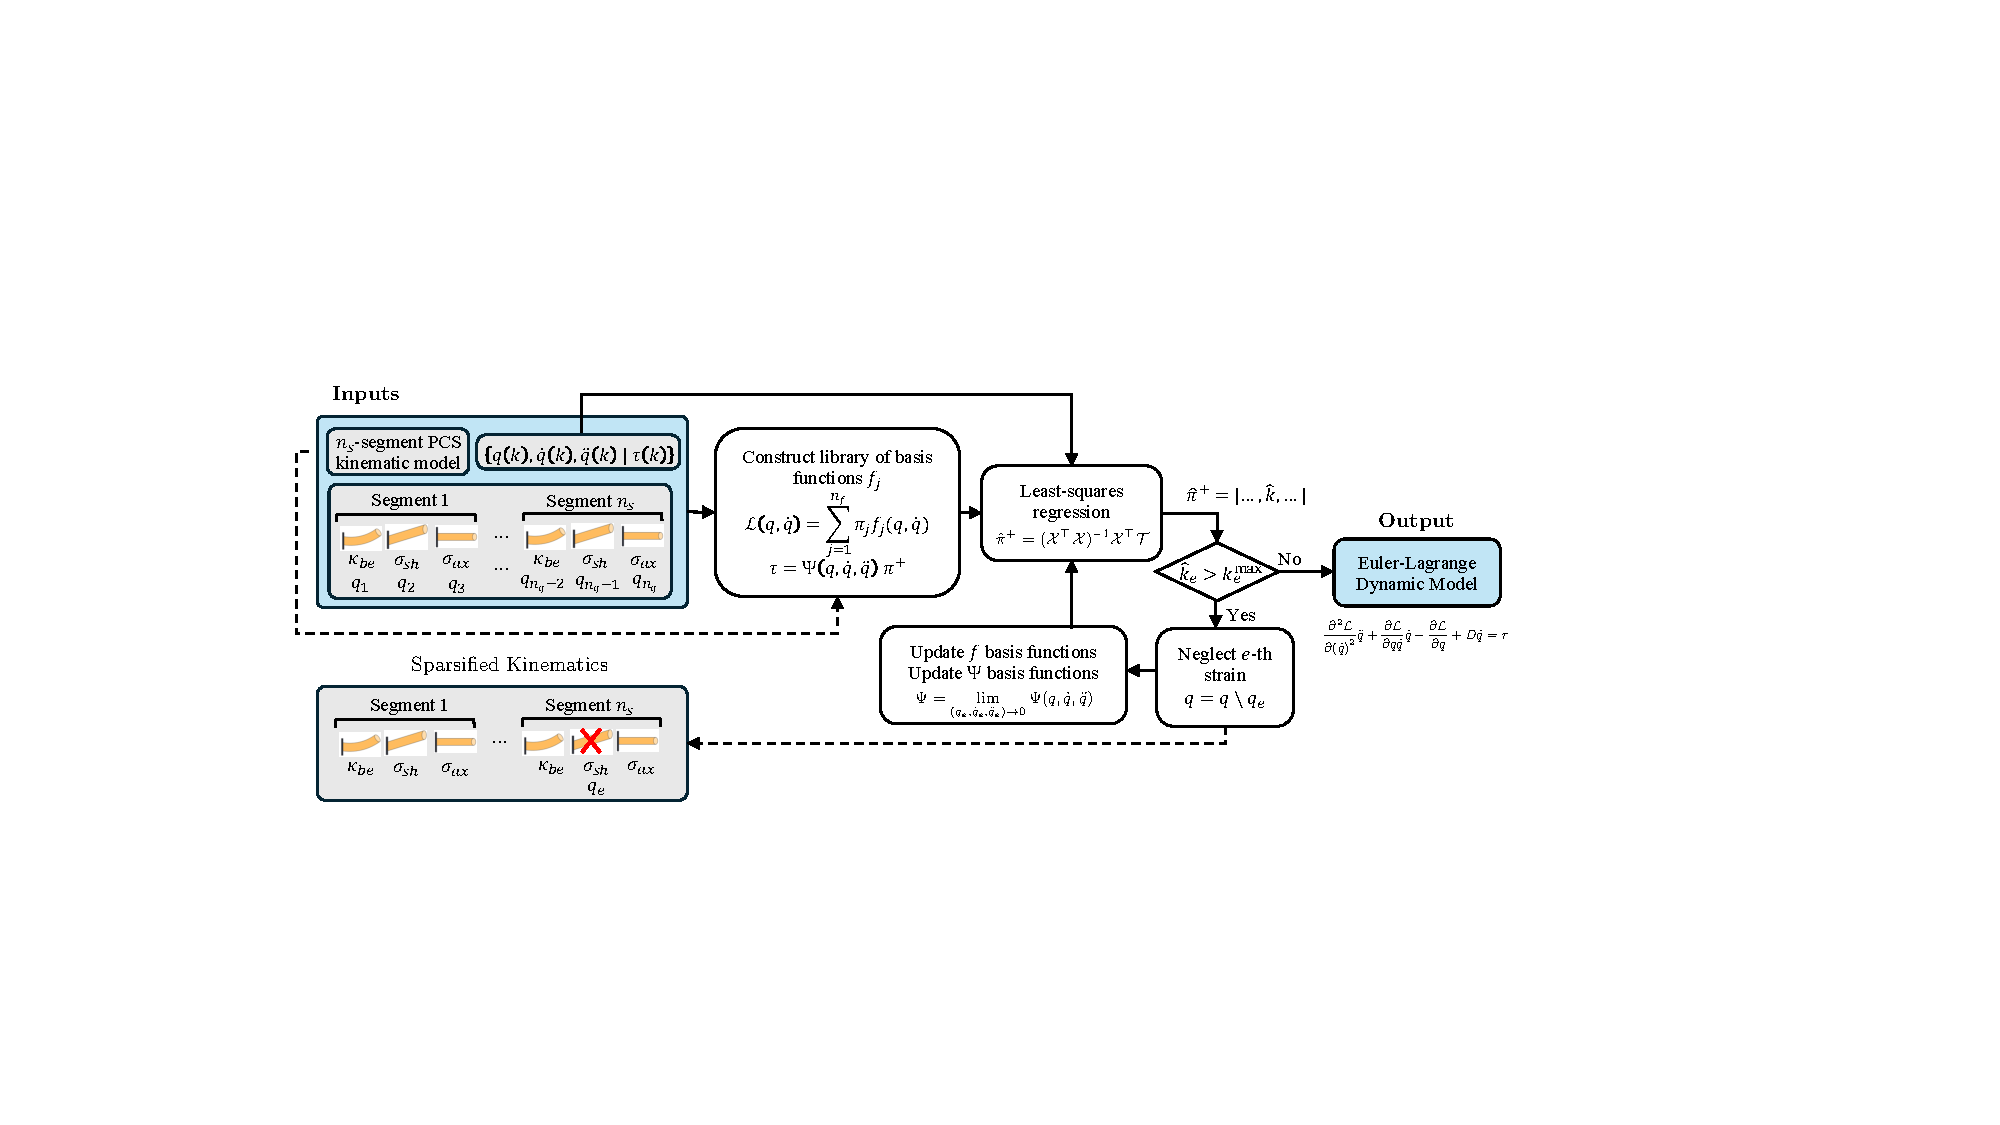
\includegraphics[width=1.0\linewidth]{pcsregression/figures/diagram_dynamic_regression_v2_cropped.pdf}
    \caption{Schematic of the dynamic model identification process that simultaneously regresses the dynamic parameters and neglects unimportant strains. Based on a $n_\mathrm{s}$-segment \gls{PCS} model, a library of basis functions is constructed to parameterize the system’s Lagrangian and \gls{EOM}. A regression framework is established on a dataset of configuration-space positions $\dot{q}(k)$, velocities $\dot{q}(k)$, accelerations $\ddot{q}(k)$, and actuation torques $\tau(k)$ that estimates the dynamic parameters $\hat{\pi}^+$ with closed-form, linear least squares. Strains that exhibit a stiffness higher than a predefined threshold are neglected, prompting adjustments to the basis functions. Subsequently, this procedure is repeated until all strain stiffnesses lie below the threshold.}
    \label{fig:pcsregression:dyn_regr}
\end{figure}

\subsection{Dynamic Regression \& Strain Sparsification}
After obtaining a kinematic model with the \emph{Kinematic Fusion} algorithm, we can employ the identified parametrization as a foundation for deriving a dynamic model. % To do so, we implement a data-driven dynamic identification method that allows the extraction of a minimalistic-dimensional description of a soft manipulator.
First, we symbolically derive the basis functions of the \gls{PCS} dynamical model.
Subsequently, we implement an iterative procedure to (i) regress dynamic coefficients with linear least squares and (ii) identify strains that can be neglected and remove them from the dynamical model.

\subsubsection{Parametrization of the PCS Dynamic Model with Basis Functions}
In order to easily regress the dynamic parameters with linear least squares, we first derive the \gls{PCS} dynamics for a $n_\mathrm{s}$ segment soft robot from first principle~\citep{armanini2023soft, della2023model}, with all rotational and linear strains taken into account, and subsequently parametrize both the Lagrangian and Euler-Lagrangian equations as a linear combination of monomial basis function.
% In this work, we will perform a system identification to find the Lagrangian of the soft robot. Let us consider a soft manipulator with configuration variables $q \in \mathbb{R}^{n_q}$. We leverage the knowledge of the previously found kinematic model to parametrize the Lagrangian as a linear combination of monomial basis functions,
\begin{equation}\label{eq:pcsregression:lagrangian_basis_functions}
    \mathcal{L}(q, \dot{q}) = \sum_{j=1}^{n_\mathrm{f}} \pi_j f_j(q, \dot{q}), 
    \quad
    \tau = \sum_{j=1}^{n_\Psi} \pi_j^{+}\Psi_j(q,\dot{q},\ddot{q}) \in \mathbb{R}^{n_q},
\end{equation}
where $f_j: \mathbb{R}^{n_\mathrm{q}} \times \mathbb{R}^{n_\mathrm{q}} \to \mathbb{R}$ denotes each of the basis functions, and $\pi \in \mathbb{R}^{n_\mathrm{f}}$ the corresponding coefficients.
Analog, we derive symbolically the \gls{EOM} using an Euler-Lagrangian approach (see Section~\ref{sub:pcsregression:lagr_dynamics}) and now state the corresponding basis functions as $\Psi(q, \dot{q}, \ddot{q}) \in \mathbb{R}^{n_\Psi \times n_\mathrm{q}}$ with $\Psi_j: \mathbb{R}^{n_\mathrm{q}} \times \mathbb{R}^{n_\mathrm{q}} \times \mathbb{R}^{n_\mathrm{q}} \to \mathbb{R}^{n_\mathrm{q}}$ such that
\begin{equation}
    \tau = \sum_{j=1}^{n_{f}} \left[ \pi_j \left( \diffp[2]{f_j}{{\dot{q}}}\ddot{q} + \diffp{f_j}{{q}{\dot{q}}}\dot{q} - \diffp{f_j}{{q}} \right) \right] + D\dot{q},
\end{equation}
where
$\pi^+ = \begin{bmatrix}
    \pi^\top & d^\top 
\end{bmatrix}^\top \in \mathbb{R}^{n_{\Psi}}$ contains the associated coefficients and consists of $\pi$ and the damping coefficients $d = \mathrm{diag}(D) \in \mathbb{R}^{n_\mathrm{q}}$.

\subsubsection{Regression of Dynamic Parameters}\label{ssub:pcsregression:reg_dyn_params}
In order to estimate the dynamic coefficients, we formulate the linear regression problem as $\mathcal{T}=X \pi^+$, which accommodates the dataset of positions, velocities, and accelerations 
$\mathcal{X} = [\Psi(q(1), \dot{q}(1), \ddot{q}(1))^{\top},...,\Psi(q(T), \dot{q}(T), \ddot{q}(T))^{\top}]^{\top} \in \mathbb{R}^{T n_\mathrm{q} \times n_{\Psi}}$ 
% \begin{equation}
%     \mathcal{X} = [\Psi(q(1), \dot{q}(1), \ddot{q}(1))^{\top}, \dots, \Psi(q(T), \dot{q}(T), \ddot{q}(T))^{\top}]^\top \in \mathbb{R}^{T n_\mathrm{q} \times n_{\Psi}}
% \end{equation}
and the corresponding actuation inputs 
% $\mathcal{T} = \begin{bmatrix}
%     \tau^{\top}(1), & \dots, & \tau^{\top}(T)
% \end{bmatrix}^{\top} \in \mathbb{R}^{T n_\mathrm{q}}$.
$\mathcal{T}=[\tau^{\top}(1), \dots,\tau^{\top}(T)] \in \mathbb{R}^{T n_\mathrm{q}}$. 
We solve this optimization problem with linear least squares, which minimizes the residual error as $\min \lVert \mathcal{T} - \mathcal{X} \, \pi^+ \rVert_2^2$ and allows us to identify the dynamic model coefficients in closed form as
\begin{equation}
    \hat{\pi}^+ = (\mathcal{X}^{\top} \, \mathcal{X})^{-1} \, \mathcal{X}^{\top} \mathcal{T}.
\end{equation}

\subsubsection{Sparsification of Strains}\label{ssub:pcsregression:strain_spars}
This dynamic identification method offers the advantage of having interpretable results, as each estimated coefficient has some physical meaning within the \gls{PCS} dynamic derivation. Specifically, among those we can extract the estimated stiffness matrix $\hat{K} = \mathrm{diag}(\hat{k}_1, \dots, \hat{k}_{n_\mathrm{q}})$, allowing us to assess the importance of each strain through its stiffness magnitude $\hat{k}_e$. A strain with high stiffness usually exhibits low displacement, approximating rigid behavior. Therefore, such strain can be considered non-essential and neglected in the dynamics.
We define a maximum allowable stiffness $k^\mathrm{max}_e \in \mathbb{R}_{\geq0}$ for each strain/configuration variable as a function of the maximum Elastic and Shear moduli $E^{\text{max}}, G^{\text{max}} \in \mathbb{R}_{\geq 0}$. For example, in the planar case and for constant cross sections of area $A_\mathrm{c}$ and second moment of inertia $I_\mathrm{c}$, this can be conveniently done as
% For this, we define a maximum stiffness, which is commonly modeled using the cross-section geometry and the material properties \citep{shi2024stiffness}. For a planar segment with constant cross-section, this is given by
\begin{equation}
    k_{\mathrm{be}}^{\mathrm{max}} = I_c E^{\mathrm{max}},
    \quad
    k_{\text{sh}}^{\text{max}} = A_c G^{\mathrm{max}},
    \quad
    k_{\text{ax}}^{\text{max}} = A_c E^{\text{max}}.
\end{equation}

Given these maximum stiffnesses, the $e$-th strain is neglected if its estimated stiffness lies above the threshold $\hat{k}_e>k_e^{\mathrm{max}}$. Therefore, the $e$-th strain is removed as a configuration variable through
% $q = q\setminus q_e$, 
\begin{equation}
    q' = \begin{bmatrix}
        q_1, q_2, \ldots, q_{e-1}, q_{e+1}, \ldots, q_{n_\mathrm{q}})
    \end{bmatrix}^\top,
\end{equation}
and its influence on the dynamics needs to be eliminated as well. We update the Euler-Lagrange basis functions as $\Psi = \lim_{(q_e,\dot{q}_e,\ddot{q}_e)\to 0} \Psi (q, \dot{q}, \ddot{q})$. Any columns that turn into all-\emph{zeros} are also removed, and the coefficient vector $\pi^+$ is updated accordingly by removing the corresponding rows. A similar procedure applies to the Lagrangian basis functions $f$ and their coefficients $\pi$.

% Having reached this result, we must perform a new regression of the parameters to find the sparser dynamic model. For this, the configuration vector is updated by excluding the $e$-th strain $q_e$ ($q=q\setminus q_e$), and the Lagrangian basis functions are adjusted such that the updated Lagrangian parameterization is given by
% \begin{align}\label{eq:pcsregression:update_basis_fcns}
%     \mathcal{L}(q,\dot{q}) = \sum_{j=1}^{n_{f}} \pi_j \lim_{(q_e,\dot{q}_e)\to 0} f_j (q,\dot{q}) \,.
% \end{align}
% Similarly, the Euler-Lagrange basis functions $\Psi$ can be updated by removing the $e$-th row and taking the following limit to the remaining entries, 
% \begin{align}
%     \lim_{(q_e,\dot{q}_e,\ddot{q}_e)\to 0} \Psi (q, \dot{q}, \ddot{q})\,.
% \end{align}
% Any columns that turn into all-\emph{zeros} are also removed. 

This procedure of regressing dynamic coefficients and sparsifying strains, as presented in Sections~\ref{ssub:pcsregression:reg_dyn_params} and \ref{ssub:pcsregression:strain_spars}, respectively, is the number of strains/configuration variables converges (i.e., remains constant). We stress that the (likely) computationally expensive operation of symbolically deriving the library of basis functions only needs to be done once at the beginning, as we subsequently update the library by taking the limit at the end of each iteration.

% Notice, therefore, that the library of basis functions is only derived once in the beginning, considering all possible strains. Later, in case of strain removal, only the above adjustments are performed to the set. After this, linear least squares are used to find the new set of parameters. The sequence of steps described in \ref{ssub:pcsregression:reg_dyn_params} and \ref{ssub:pcsregression:strain_spars} is repeated until the stiffness threshold produces no effects. %Algorithm \ref{} summarizes the steps taken to find this dynamic model.
